% ============================================================================
% Course Wrap-Up and Outlook
% University of Padova, 23-24 September 2026
% April 20--23 & May 4--7, 2026
% Duration: 25 minutes
% ============================================================================

\documentclass[aspectratio=169,11pt]{beamer}

% ---------- Theme and colors ----------
\usecolortheme{dove}
\setbeamertemplate{navigation symbols}{}
\setbeamertemplate{footline}{%
  \hfill\usebeamerfont{page number in head/foot}%
  \usebeamercolor[fg]{normal text}%
  \insertframenumber\,/\,\inserttotalframenumber\kern1em\vskip4pt}
\setbeamerfont{frametitle}{size=\huge}

% ---------- Packages ----------
\usepackage[utf8]{inputenc}
\usepackage[T1]{fontenc}
\usepackage{amsmath,amssymb,amsfonts}
\usepackage{bm}
\usepackage{graphicx}
\graphicspath{{fig/}}
\usepackage{tikz}
\usetikzlibrary{shapes,arrows.meta,positioning,calc,fit,backgrounds,patterns,decorations.pathreplacing}
\usepackage{booktabs}
\usepackage{hyperref}
\usepackage{xcolor}

% ---------- Custom colors ----------
\definecolor{uzhblue}{rgb}{0,0,0.5}
\definecolor{uzhgreylight}{RGB}{236,238,241}
\definecolor{uzhgreydark}{RGB}{81,86,94}
\definecolor{harvardcrimson}{RGB}{153,0,0}
\definecolor{unil@blue}{RGB}{0,140,204}
\definecolor{unil@black}{RGB}{35,31,32}
\definecolor{darkgreen}{RGB}{0,100,0}
\definecolor{darkred}{RGB}{139,0,0}
\definecolor{softblue}{RGB}{70,130,180}
\definecolor{softorange}{RGB}{230,159,0}
\definecolor{softgreen}{RGB}{0,158,115}

% ---------- Set beamer colors ----------
\setbeamercolor{frametitle}{bg=uzhgreylight, fg=uzhblue}
\setbeamercolor{title}{fg=uzhblue}
\setbeamercolor{structure}{fg=uzhblue}
\setbeamercolor{block title}{bg=unil@blue, fg=white}
\setbeamercolor{block body}{bg=uzhgreylight}
\setbeamercolor{block title alerted}{bg=darkred,fg=white}
\setbeamercolor{block body alerted}{bg=red!5}
\setbeamercolor{block title example}{bg=darkgreen,fg=white}
\setbeamercolor{block body example}{bg=green!5}
\setbeamercolor{item}{fg=unil@black}
\setbeamercolor{normal text}{fg=unil@black}

% ---------- Emphasis and hyperlinks ----------
\newcommand{\emphc}[1]{\textcolor{harvardcrimson}{#1}}
\hypersetup{colorlinks,linkcolor=harvardcrimson,urlcolor=harvardcrimson}

% ---------- Math commands ----------
\newcommand{\R}{\mathbb{R}}
\newcommand{\E}[1]{\mathbb{E}\!\left[#1\right]}

% ---------- Title ----------
\title[Wrap-up -- Padova 2026]%
{Deep Learning for Solving Dynamic Models}
\subtitle{Wrap-up: what to use when, and what to watch out for}
\author{Simon Scheidegger}
\institute[HEC Lausanne]{HEC, University of Lausanne}
\date{University of Padova\\September 24, 2026}

\begin{document}

{\setbeamercolor{background canvas}{bg=uzhgreylight}
\begin{frame}
\titlepage
\end{frame}
}
\begin{frame}{The Big Picture: One Computational Paradigm}
\begin{center}
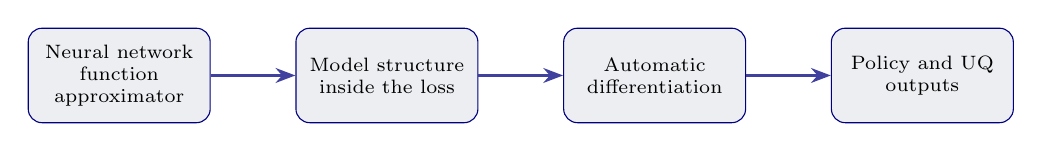
\begin{tikzpicture}[
    box/.style={rectangle, draw=uzhblue, fill=uzhgreylight, rounded corners=5pt,
                text width=2.1cm, minimum height=1.2cm, align=center, font=\scriptsize,
                inner sep=3pt},
    arr/.style={-{Stealth[length=2.5mm]}, very thick, uzhblue!75}
]
\node[box] (nn)     at (0,0)    {Neural network\\function approximator};
\node[box] (loss)   at (3.4,0)  {Model structure\\inside the loss};
\node[box] (ad)     at (6.8,0)  {Automatic\\differentiation};
\node[box] (policy) at (10.2,0) {Policy and UQ\\outputs};

\draw[arr] (nn.east)   -- (loss.west);
\draw[arr] (loss.east) -- (ad.west);
\draw[arr] (ad.east)   -- (policy.west);
\end{tikzpicture}
\end{center}

\vspace{0.25cm}
\begin{block}{Across methods}
DEQN, PINN, deep surrogates, and GP-BAL differ in objective and geometry,\\
but share the same core optimization logic.
\end{block}
\end{frame}


\begin{frame}{Course Arc: Two Days}
\small
\begin{center}
\begin{tabular}{ll}
\toprule
\textbf{Session} & \textbf{Step in the pipeline} \\
\midrule
1 & Deep learning foundations, optimization, and generalization \\
2 & DEQNs: equilibrium residuals as an unsupervised loss (Brock--Mirman) \\
3 & Scaling to a 2N-dimensional state space (IRBC) \\
4 & Making training work: architecture search and loss balancing \\
5 & Cohort structure and constraints (OLG, 56 generations) \\
6 & Amortizing the solve: deep surrogates and Gaussian processes \\
7 & Structural estimation via SMM on top of a surrogate \\
8--9 & Continuous time: PINNs for ODEs, PDEs, HJB and option pricing \\
\bottomrule
\end{tabular}
\end{center}

\vspace{0.2cm}
\begin{alertblock}{Main message}
The toolkit is modular: solve the model, amortize the solve, then estimate,
each layer reuses the one below it.
\end{alertblock}
\end{frame}

\begin{frame}{Visual Timeline of the Course Workflow}
\begin{center}
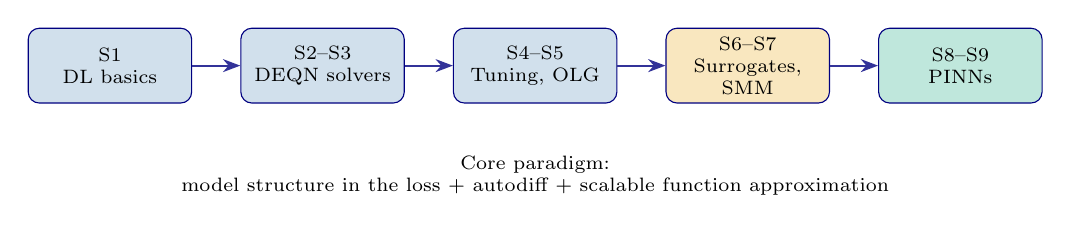
\begin{tikzpicture}[
    phasebox/.style={rectangle, draw=uzhblue, rounded corners=4pt, text width=1.9cm,
                 minimum height=0.95cm, align=center, fill=uzhgreylight, font=\scriptsize,
                 inner sep=2.5pt},
    arr/.style={-{Stealth[length=2.2mm]}, thick, uzhblue!80}
]
\node[phasebox, fill=softblue!25]   (s1) at (0,0)    {S1\\DL basics};
\node[phasebox, fill=softblue!25]   (s2) at (2.7,0)  {S2--S3\\DEQN solvers};
\node[phasebox, fill=softblue!25]   (s4) at (5.4,0)  {S4--S5\\Tuning, OLG};
\node[phasebox, fill=softorange!25] (s6) at (8.1,0)  {S6--S7\\Surrogates, SMM};
\node[phasebox, fill=softgreen!25]  (s8) at (10.8,0) {S8--S9\\PINNs};

\draw[arr] (s1.east) -- (s2.west);
\draw[arr] (s2.east) -- (s4.west);
\draw[arr] (s4.east) -- (s6.west);
\draw[arr] (s6.east) -- (s8.west);

\node[font=\scriptsize, align=center] at (5.4,-1.4)
  {Core paradigm:\\model structure in the loss $+$ autodiff $+$ scalable function approximation};
\end{tikzpicture}
\end{center}
\end{frame}

\begin{frame}{Decision Guide: Which Method When?}
\scriptsize
\begin{center}
\begin{tabular}{p{0.17\textwidth}p{0.32\textwidth}p{0.32\textwidth}}
\toprule
\textbf{Method} & \textbf{Use case} & \textbf{Strength} \\
\midrule
DEQN & Recursive equilibrium with explicit Euler residuals & Scales to high-dimensional states \\
PINN & Continuous-time PDE / HJB / KFE systems & Mesh-free; no tensor grid to refine \\
Finite difference & Low-dimensional continuous-time problems & Fast, accurate, well understood \\
Deep surrogate & Expensive simulator queried many times & Amortizes the solve; differentiable \\
GP $+$ BAL & Smooth low/medium-dimensional maps & Built-in UQ and sample efficiency \\
\bottomrule
\end{tabular}
\end{center}

\vspace{0.2cm}
\begin{block}{Rule of thumb}
Reach for a neural method when the state space defeats a tensor grid,
not before. In two or three dimensions the classical solver usually wins.
\end{block}
\end{frame}
\begin{frame}{Common Failure Modes and Mitigations}
\small
\begin{columns}[T]
\column{0.49\textwidth}
\textbf{Failure modes}
\begin{itemize}
    \item Calibration mismatch to benchmark science
    \item Training focused on wrong state regions
    \item Over-reliance on mean loss diagnostics
    \item Surrogate extrapolation outside training support
\end{itemize}

\column{0.49\textwidth}
\textbf{Mitigations}
\begin{itemize}
    \item Explicit benchmark tests and stress scenarios
    \item Mixed exogenous/endogenous sampling
    \item Report residual distributions and constraints
    \item Active learning and uncertainty-aware evaluation
\end{itemize}
\end{columns}
\end{frame}

\begin{frame}{Implementation Checklist}
\small
\begin{enumerate}
    \item Define state/control vectors and feasibility transforms.
    \item Engineer residual blocks from economics and climate equations.
    \item Set sampling scheme and training diagnostics before tuning architecture.
    \item Validate on out-of-sample simulations and benchmark moments.
    \item Build surrogate/UQ layer only after solver quality is verified.
    \item Separate normative objective from political/participation constraints.
\end{enumerate}
\end{frame}


\begin{frame}{What We Did Not Cover}
\small
Each of these is a natural next step from where we stopped:
\begin{itemize}\itemsep4pt
  \item \textbf{Sequence-space DEQNs}: transition paths and MIT shocks.
  \item \textbf{Krusell--Smith and Young's method}: a continuum of agents with
        a distribution as a state variable.
  \item \textbf{Climate economics and IAMs}: DICE with DEQNs, deep uncertainty
        quantification, constrained Pareto-improving carbon taxes.
  \item \textbf{Continuous-time heterogeneous agents}: the coupled HJB--KFE system,
        continuous-time Aiyagari, and the master equation.
  \item \textbf{Agentic programming}: AI coding agents as research partners.
\end{itemize}
\end{frame}

\begin{frame}{Research Frontier}
\begin{itemize}\itemsep4pt
  \item Richer heterogeneity: regional, sectoral, and household dimensions.
  \item Estimation at scale: likelihood-based and simulation-based inference
        on top of amortized solvers.
  \item Better theoretical guarantees: convergence, error bounds, and
        verification of trained policies.
  \item Operator learning: mapping whole parameterizations to solutions,
        rather than one model at a time.
  \item Robustness: model ensembles and policy design under ambiguity.
\end{itemize}
\end{frame}

\begin{frame}{Closing Message}
\begin{block}{From method to model}
These methods earn their place when they make a model \emphc{tractable} that was
not, without giving up the \emphc{diagnostics} that let you trust the answer.
Always keep a benchmark you can check against.
\end{block}

\vspace{0.5cm}
\begin{center}
{\Large Thank you for participating in the course.}\\[6pt]
{\LARGE \emphc{Questions and discussion}}
\end{center}
\end{frame}

\end{document}
